\section{An implementation of no-slip boundary conditions in DPD}
\subsection{模型}
\frame{\frametitle{模型}
\begin{columns}
\begin{column}[c]{0.5\textwidth}
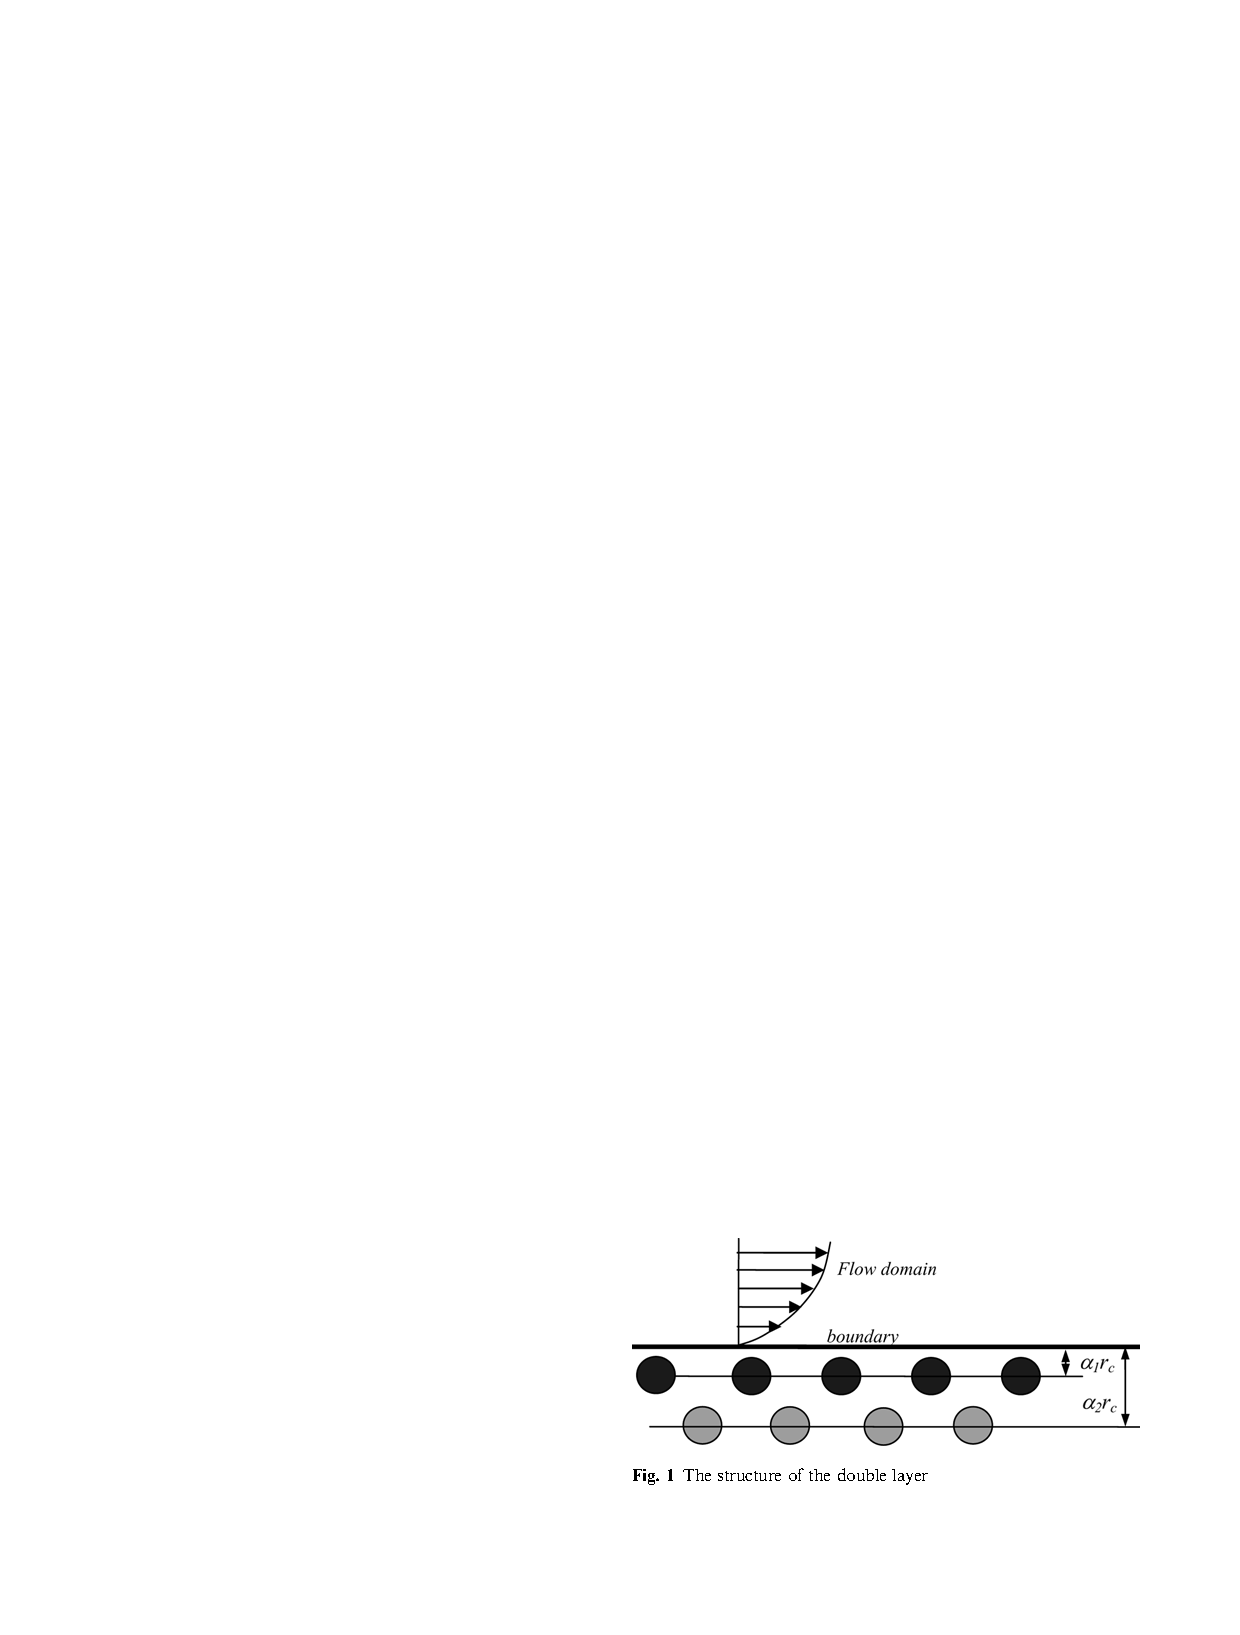
\includegraphics[width=1\textwidth]{./figures/fig11.pdf}
\end{column}
\begin{column}[c]{0.5\textwidth}
$\alpha_1$,$\alpha_2$满足:
\[
0<\alpha_1<\alpha_2
\]

穿过边界的粒子
\[
v_{new} = 2v_{wall} - v_{old}
\]
\[
r_{new} = r_{old} + 2d_r\mathbf{n_w}
\]
\end{column}
\end{columns}
}

\subsection{结果}
\frame{\frametitle{边界单粒子层}
\begin{center}
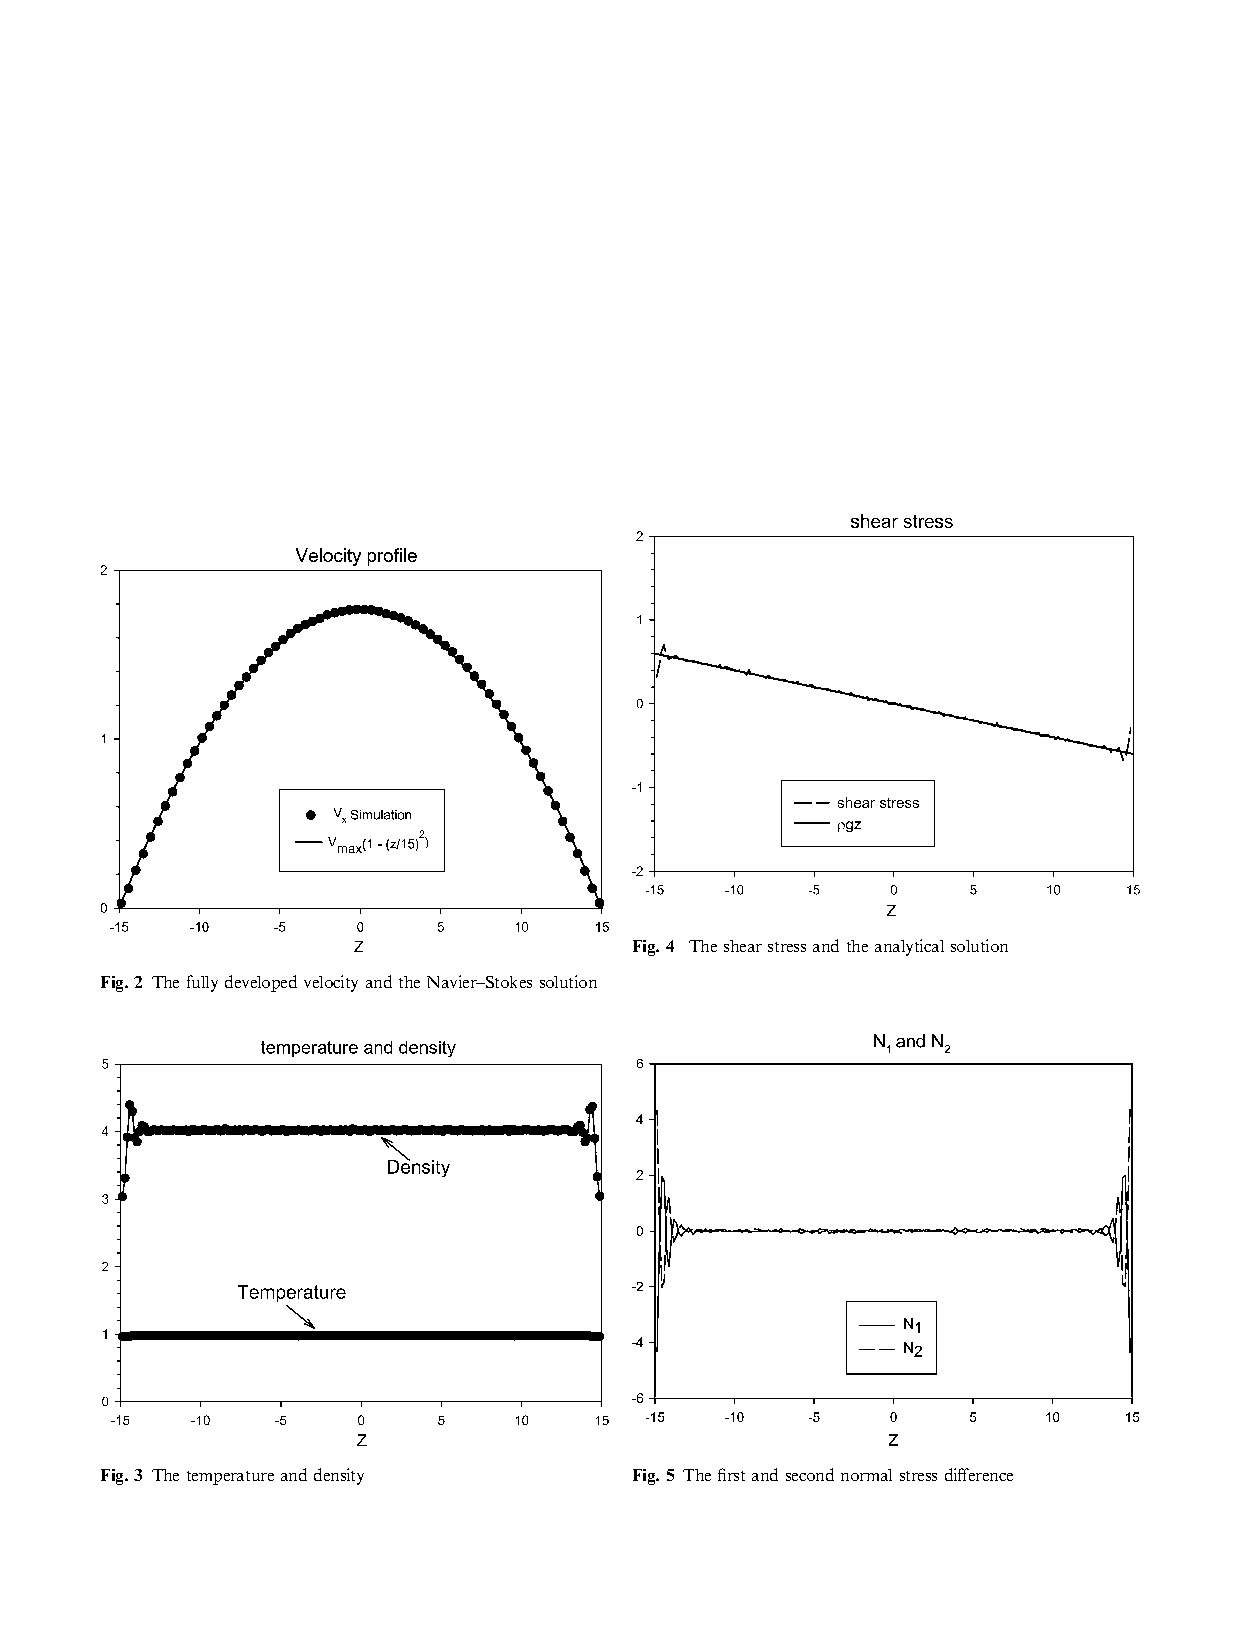
\includegraphics[width=0.7\textwidth]{./figures/fig12.pdf}
\end{center}
}

\frame{\frametitle{边界双粒子层}
\begin{columns}
\begin{column}[c]{0.5\textwidth}
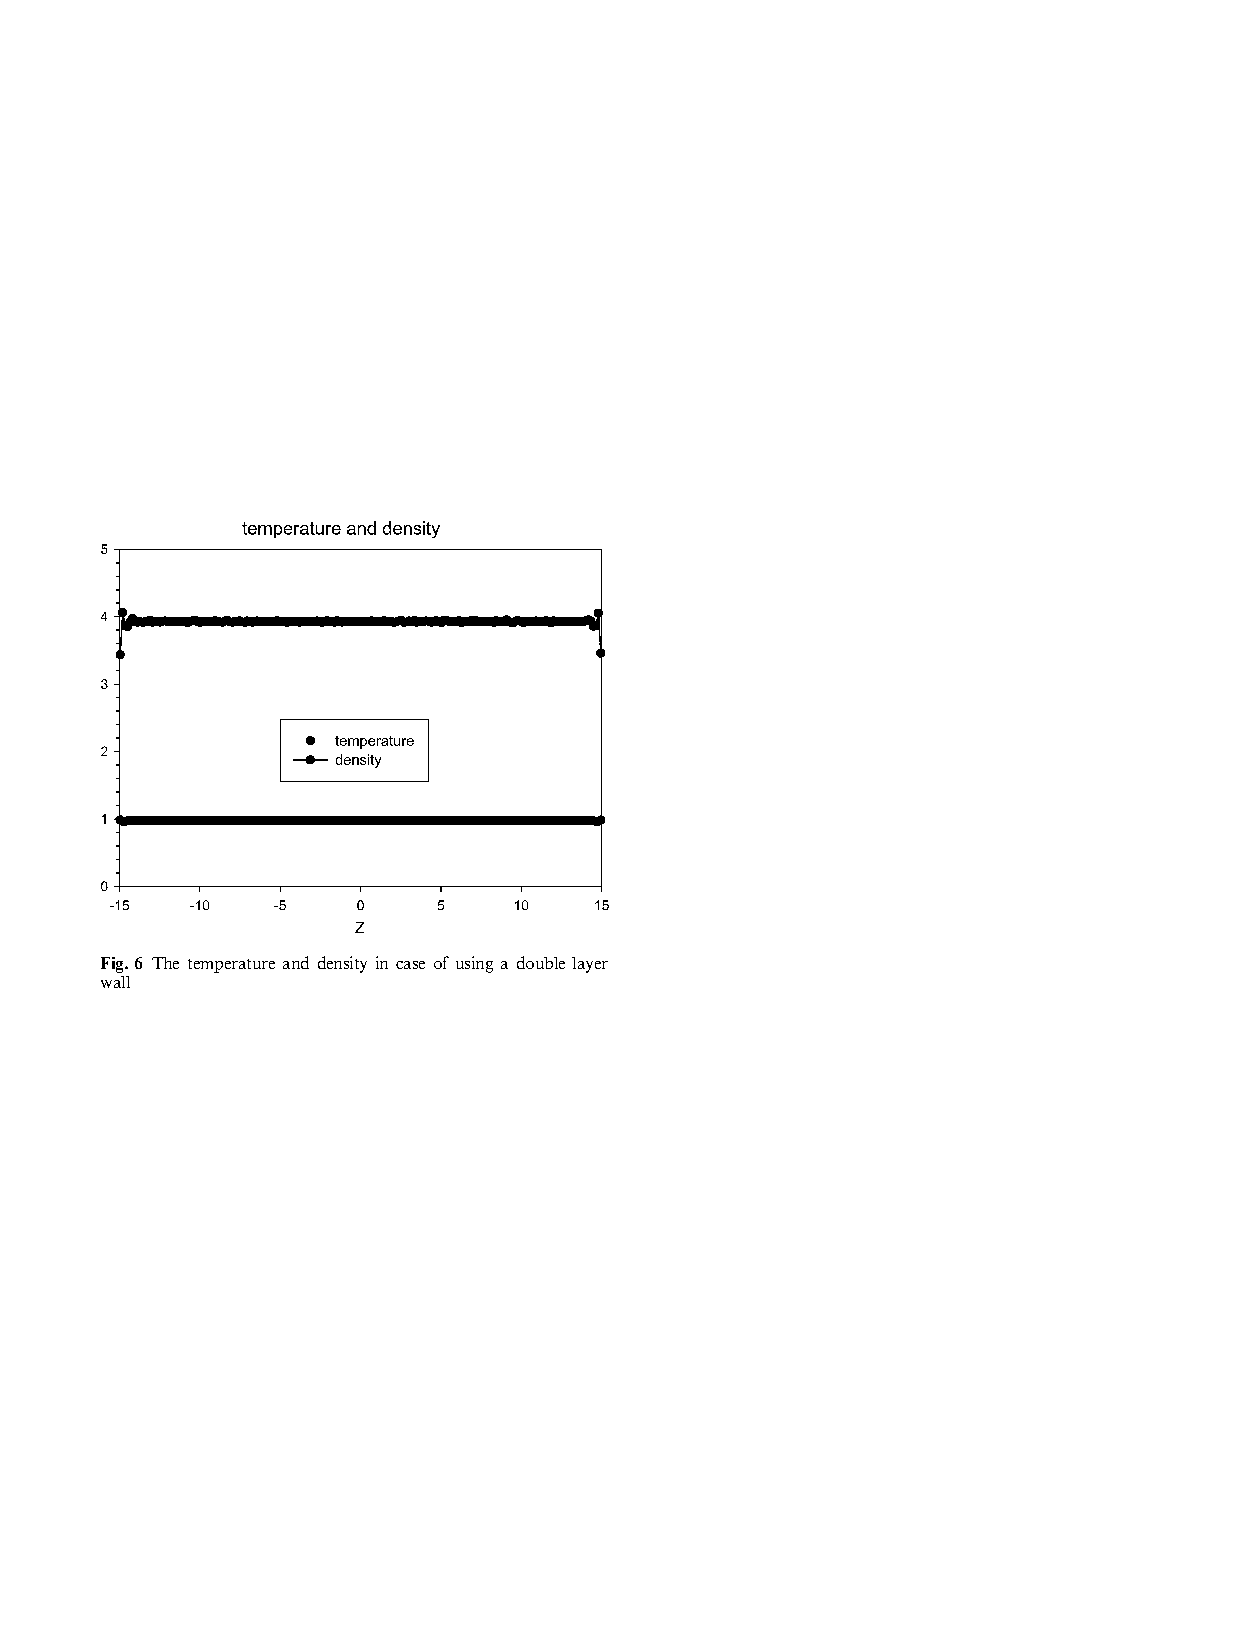
\includegraphics[width=1\textwidth]{./figures/fig13.pdf}
\end{column}
\begin{column}[c]{0.5\textwidth}
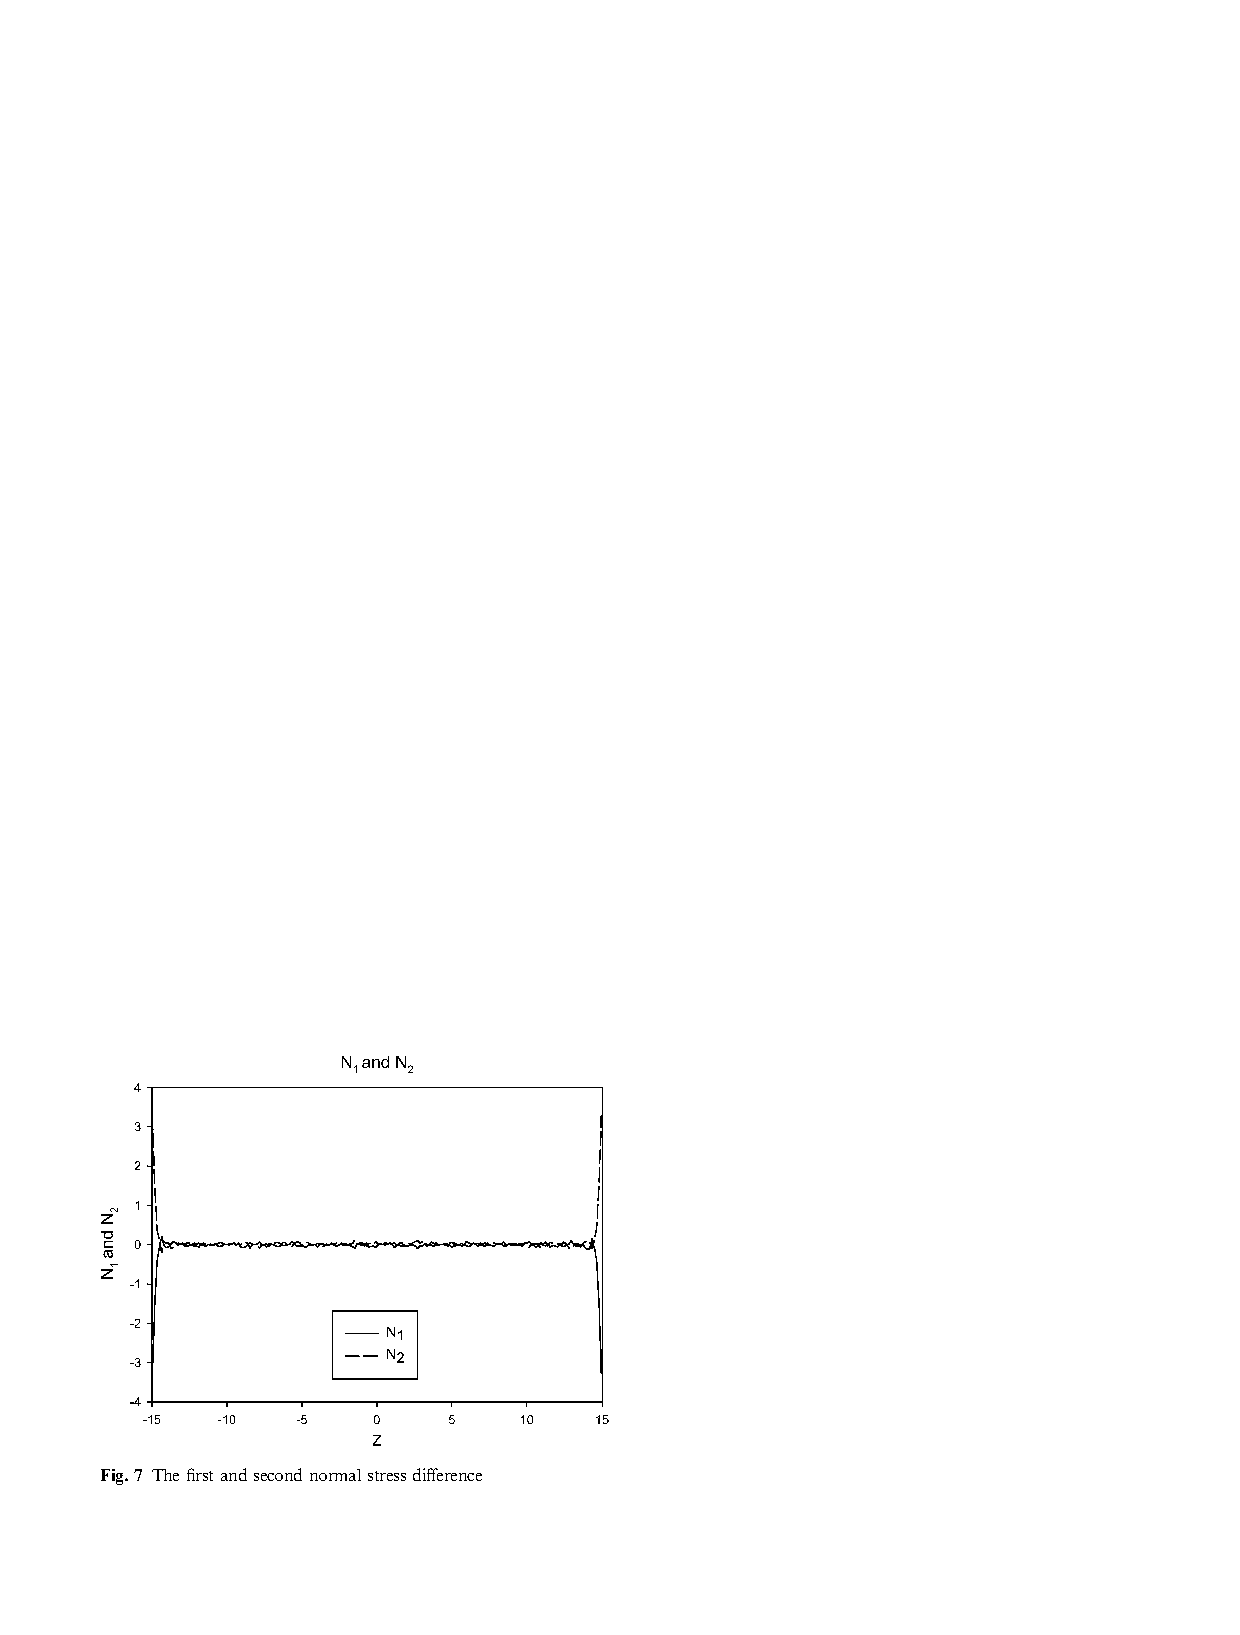
\includegraphics[width=1\textwidth]{./figures/fig14.pdf}
\end{column}
\end{columns}
}
